\documentclass[CJK]{beamer}

\usepackage{CJK}
\usepackage{color}
\usepackage{graphicx}
\usepackage{listings}
\usepackage{xcolor}
\lstset{
	%行号
		%numbers=left,
		%背景框
			%framexleftmargin=10mm,
		%frame=none,
		%背景色
			%backgroundcolor=\color[rgb]{1,1,0.76},
		backgroundcolor=\color[RGB]{245,245,244},
		%样式
			keywordstyle=\bf\color{blue},
		identifierstyle=\bf,
		numberstyle=\color[RGB]{0,192,192},
		commentstyle=\it\color[RGB]{0,96,96},
		stringstyle=\rmfamily\slshape\color[RGB]{128,0,0},
		%显示空格
			showstringspaces=false
}

\hypersetup{CJKbookmarks=true}
%\usetheme{PaloAlto}
\usetheme{CambridgeUS}
\usefonttheme[onlymath]{serif}

\newcommand\song{\fontspec{宋体}}
\newcommand\hei{\fontspec{黑体}}
\newcommand\kai{\fontspec{楷体\_GB2312}}
\newcommand\lishu{\fontspec{隶书}}
\newcommand\yahei{\fontspec{微软雅黑}}

\begin{document}
\begin{CJK}{UTF8}{gbsn}

\title[Simulator]{\huge Unicore Simulator 结题报告}
\author{李春奇 \and 彭焯 \\ 王kan \and 华连盛}
\date{\today}
\institute{PKU}

\begin{frame}
\titlepage
\end{frame}

%%%%%%%%%%%%%%%%%%%%%%%%%%%%%%%%%%%
\section*{目录}

\begin{frame}
\hypertarget{Contents}
\frametitle{Contents}
\tableofcontents[pausesection]
\end{frame}

%%%%%%%%%%%%%%%%%%%%%%%%%%%%%%%%%%
\section{工程概述}

\begin{frame}
\huge{工程概述}
\end{frame}

\subsection{设计目标}
\begin{frame}
	\frametitle{设计目标}
	开题报告中所设定的设计目标:
	\begin{itemize}
		\item 模拟五级流水的流水线CPU设计。
		\item 模拟至少一级cache,采用哈佛结构
		\item 模拟动态内存管理
		\item 一些库函数的模拟器级别的实现
		\item 调试工具的实现和CPU性能的统计
	\end{itemize}
	附加完成的功能:
	\begin{itemize}
		\item 反汇编模块的支持。
		\item 多种模式的支持(验证模式和自动运行模式)。
	\end{itemize}
\end{frame}

%%%%%%%%%%%%%%%%%%%%%%%%%%%%%%%%%%
\section{项目介绍}

\begin{frame}
	\huge{项目介绍}
\end{frame}

\subsection{项目视图}
\begin{frame}
	\frametitle{项目模块视图}
	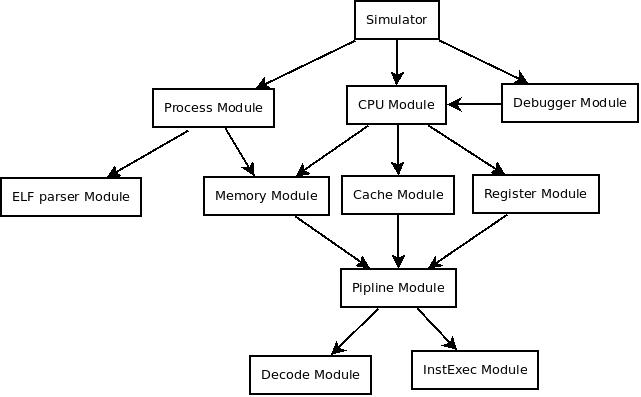
\includegraphics[height=4.5cm]{module_view.jpeg}
\end{frame}


\subsection{CPU 模块}
\begin{frame}[fragile]
	\frametitle{CPU 模块}
	CPU模块是Simulator中最重要的模块,是整个Simulator的核心。CPU模块由两个子模块构成:进程模块和流水线模块。
	\begin{itemize}
		\item 进程模块负责ELF文件的解析、进程控制块(PCB)的初始化、进程内存空间的初始化。
		\item 流水线模块是CPU模块的核心,模拟了CPU的五级流水,实现了互锁和数据前递。
	\end{itemize}
\end{frame}

\begin{frame}[fragile]
	\frametitle{流水线}
	流水线的每一级说明如下:
	\begin{enumerate}
		\item IF-取指级:在I-cache取得指令并读入对应流水级的寄存器(具体实现为一个结构)。
		\item ID-译码与访问寄存器级:对IF级取得的指令进行译码,获得指令类型、指令各域的值,存入对应流水级的寄存器中。
		\item Ex-指令执行级:对ALU指令进行运算,跳转指令和访存指令进行计算跳转地址和存储地址。对ALU类指令做数据前递。
		\item Mem-访存级:对访存类指令进行内存的存取。取内存指令在这一级实现前递,并标记需要互锁的寄存器。
		\item WR-写回级:将目的寄存器写回。
	\end{enumerate}
\end{frame}

\begin{frame}[fragile]
	\frametitle{流水线互锁}
	\begin{itemize}
		\item 五级流水的互锁主要是Load指令和随后用到该指令目的寄存器的指令间会产生数据相关冒险。在模拟器的实现中,若遇到数据相关,则IF、ID级流水需要暂停一拍并在Ex级插入一个气泡。
	\end{itemize}
	下面是互锁在模拟器中的图示:
	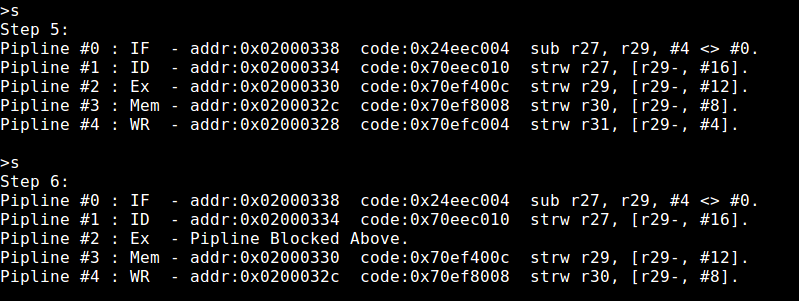
\includegraphics[height=3cm]{pipline_block.jpeg}
\end{frame}

\subsection{内存模块}
\begin{frame}[fragile]
	\frametitle{内存模块}
	Simulator实现了简单的内存管理,包括:
	\begin{itemize}
		\item 虚拟地址映射
		\item 栈空间的实现
		\item 内存访问越界检查
		\item 内存类型保护
	\end{itemize}
\end{frame}

\begin{frame}[fragile]
	\frametitle{内存模块-虚拟地址映射}
	\begin{itemize}
		\item 进程的虚拟内存按照Segment管理,第0个Segment是栈空间,之后依次为ELF文件的可载入Segment。
		\item 对于任何访问内存的请求,都必须通过虚拟内存管理的中间层,经过验证地址是否合法、访问的数据是否可读(可写)才能够进行下一步的操作。
		\item 这样的设计能够保证任何ELF文件的错误都不会导致模拟器的崩溃。
	\end{itemize}
\end{frame}

\subsection{调试模块}
\begin{frame}[fragile]
	\frametitle{断点设置模块}
	断点设置模块用来设置断点,断点地址为代码在内存中的虚拟地址。实现的功能有:
	\begin{itemize}
	\item 设置断点,并记录断点被命中的次数
	\item 删除断点
	\item 动态扩充断点集合,采用STL库中Vector的扩展方式。
	\end{itemize}
	截图如下:\\
	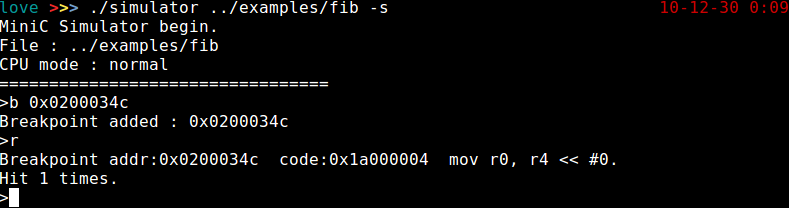
\includegraphics[height=2cm]{breakpoint.jpeg}
\end{frame}

\begin{frame}[fragile]
	\frametitle{反汇编模块}
	\begin{itemize}
		\item 反汇编模块是在计划外完成的模块,主要目的是为了便于调试,避免每次调试前都需要进行objdump获得每个指令的汇编代码。
		\item 反汇编模块能够显示从指定行开始若干行的代码,也可以显示某函数中的代码。函数名到入口地址的查询在符号表中完成。
	\end{itemize}
	截图如下:\\
	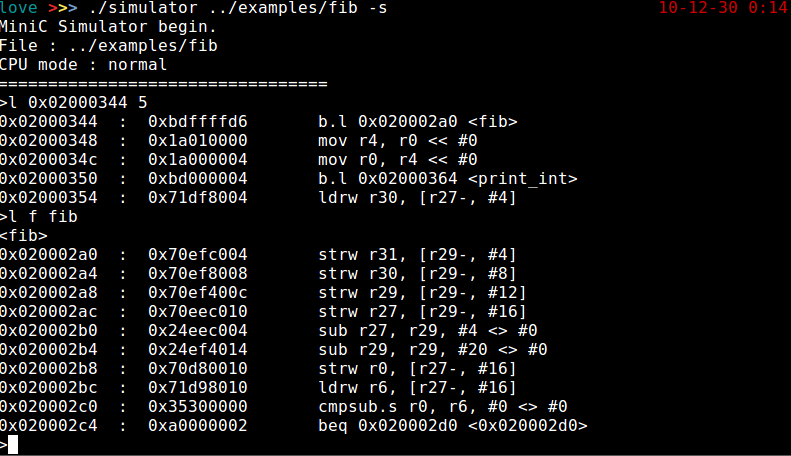
\includegraphics[height=4cm]{assemble.jpeg}
\end{frame}

\begin{frame}[fragile]
	\frametitle{统计模块}
	统计模块主要分为两个部分:CPU信息的统计和指令数信息的统计。
	\begin{itemize}
		\item CPU信息的统计主要包括CPU总周期数、空闲周期数、流水线气泡数、CACHE命中情况和访存情况。
		\item 指令数信息统计主要包括总指令数和各个类型指令数及对应比例。
	\end{itemize}
\end{frame}

\section{模拟器的特别设计}
\begin{frame}
	\frametitle{模拟器的特别设计}
	模拟器的设计过程中实现了一些计划外的独特的模块,这些模块都是用来使得模拟器的可用性更强。
	\begin{itemize}
		\item 反汇编模块的设计
		\item 断点模块的设计
		\item 内存模块的虚拟地址映射机制
		\item 对内存的修改和对寄存器的修改
		\item 对指令数及指令分类的统计
		\item 模拟器对三种模式的支持:普通模式、验证模式和自动模式
	\end{itemize}
\end{frame}

\begin{frame}
	\frametitle{模拟器的三种模式}
	模拟器支持三种模式,分别用于不同的场合。
	\begin{itemize}
		\item 普通模式:用于普通的模拟,支持单步执行、显示流水线状态、CPU状态、寄存器堆状态等,在程序结束的时候显示统计信息。
		\item 验证模式:该模式用于指令级验证模拟器的正确性,该模式下不会显示上述状态,但是会显示每步的CMSR状态和程序结束的时候显示寄存器堆状态。
		\item 自动模式:该模式不会输出任何状态信息和统计信息,只会显示程序的输出,并且会在模拟器开始的时候自动运行。该模式经过重定位之后可以自动化得到程序执行的最终结果,用于验证编译器得到的结果是否正确。脚本batch\_simulator和batch\_simulator2就是用这个模式来实现的。
	\end{itemize}
	注:batch\_simulator脚本用来验证编译器对于有正确答案的测试样例是否能够正确生成目标代码,batch\_simulator2脚本用来验证编译器对于某文件夹下的所有.c文件生成的目标代码,全部编译执行并依次输出结果。
\end{frame}

%%%%%%%%%%%%%%%%%%%%%%%%%%%%%%%%%%%%%%%%%%%%%%%%%%%%%%%%%%%
\section{模拟器验证}
\begin{frame}
	\huge{模拟器验证}
\end{frame}

\begin{frame}
	\frametitle{模拟器验证}
	模拟器的验证主要分为三个方面:
	\begin{enumerate}
		\item 函数级验证:函数级验证主要负责验证Simulator的函数调用是否正确,着重验证栈和流水线的执行状态是否正确。重点验证递归函数的调用和主函数的返回、控制流是否正确(分支循环)。
		\item 指令级验证:指令级验证主要负责验证Simulator实现的各条指令是否正确,指令验证分为三个部分:数据处理指令、分支跳转指令、访存指令,其中数据处理指令主要验证数据正确性和标志寄存器是否被正确写入,分支跳转指令主要验证跳转位置的正确性,访存指令主要验证存储器读写的正确性。
	\end{enumerate}
\end{frame}

\subsection{函数级验证}
\begin{frame}
	\frametitle{模拟器验证-函数级验证}
	函数级的验证主要验证了模拟器宏观的执行情况,主要的验证与验证代码如下:
	\begin{enumerate}
		\item 简单的main函数验证,验证代码:00simple.c
    	\item 函数调用验证,验证代码:01function.c
    	\item 递归函数调用验证,验证代码:02recursive\_func.c
    	\item if分支语句验证,验证代码:03if.c
    	\item while循环语句验证,验证代码:04while.c
    	\item for循环语句验证,验证代码:05for.c
	\end{enumerate}
\end{frame}

\subsection{指令级验证}
\begin{frame}
	\frametitle{模拟器验证-指令级验证}
	指令级验证主要验证了模拟器在执行每条指令的时候是否有正确的行为,包括寄存器的写回、CMSR的设置、cache和内存的一致性等。主要验证代码如下:\\
	数据处理指令的验证(D\_Imm\_shift、D\_Reg\_shift、D\_Immediate)
	\begin{enumerate}
		\item opcodes域的验证,验证代码:opcode.s
    	\item shift域(前两类)和Rotate域(第三类)的验证,验证代码:shift.s
    	\item S域的验证(标志寄存器设置),验证代码:cmsr\_logic.s, cmsr\_arith.s
    	\item PC作为目的寄存器的验证,验证代码:pc\_dst.s
    	\item 乘法和乘加指令的验证,验证代码:mul.s
    \end{enumerate}
\end{frame}

\begin{frame}
	\frametitle{模拟器验证-指令级验证(续)}
	分支跳转指令的验证(主要是条件转移指令的验证)
    \begin{itemize}
    	\item 对cond域的验证和跳转地址正确性的验证,验证代码:30b\_cond.c
    \end{itemize}
    访存指令的验证:\\单数据传输指令的验证、半字和有符号字传输指令的验证
    \begin{enumerate}
    	\item shift域的验证(L\_S\_R\_Offset),验证代码:40mem\_single\_shift.s
    	\item 立即数访存的验证(L\_S\_I\_Offset),验证代码:41mem\_single\_imm.s
    	\item U域、B域的验证,验证代码:42mem\_single\_U.s
    	\item S、H域的验证,验证代码:50mem\_Hw\_S\_H.s
	\end{enumerate}
\end{frame}

%%%%%%%%%%%%%%%%%%%%%%%%%%%%%%%%%%%%%%%%%
\section*{Q\&A}
\begin{frame}
	\huge Simulator整体演示
\end{frame}

\begin{frame}
  \huge Q\&A
\end{frame}


\end{CJK}
\end{document}


